\documentclass[12pt, twoside]{article}
\input{../preamble}
\usepackage{float}

\fancyhead[LO]{La Scuola d'Italia / Dr.\ Huson / IB Math \\* 27 May 2026}
\fancyhead[RO]{\fbox{\begin{minipage}{6cm}\footnotesize First \& Last name:\\[0.5cm]\end{minipage}}}
\fancyfoot[C]{\thepage}

\begin{document}
\subsubsection*{8.3 Classwork: Rational Functions as Transformations}

\noindent\emph{A graphing calculator is allowed; show your reasoning and use the GDC
to check sketches.} The \textbf{parent function} throughout is the reciprocal
function $f(x)=\tfrac{1}{x}$ (asymptotes $x=0$ and $y=0$); every function below is
built from it by \emph{translations}, \emph{reflections}, and \emph{stretches}.

\medskip

\begin{enumerate}[itemsep=0.4cm]

%--- Problem 1: translations of 1/x ---
%--- Source: informed by AA SL 2.11 transformation items (e.g. 24M.1.SL.TZ2.1, 21M.1.SL.TZ1.1) ---
\item[1.] \textbf{Translations.} Starting from the parent function $f(x)=\dfrac{1}{x}$:

\begin{enumerate}[label=(\alph*), itemsep=0.3cm]
  \item Describe fully the single transformation that maps $f$ onto
  $\displaystyle g(x)=\dfrac{1}{x+4}$.

  \vspace{1.0cm}

  \item Describe fully the single transformation that maps $f$ onto
  $\displaystyle h(x)=\dfrac{1}{x}+3$.

  \vspace{1.0cm}

  \item The function $\displaystyle p(x)=\dfrac{1}{x-2}+5$ is obtained from $f$ by
  \emph{two} translations. Describe them, and write down the equations of the
  vertical and horizontal asymptotes of $p$.

  \vspace{1.7cm}

  \item Find the $y$-intercept of $p$. Then sketch $p$ on the axes below, showing
  both asymptotes as dashed lines. Use your GDC to check the shape.
\end{enumerate}

\begin{figure}[H]
\begin{center}
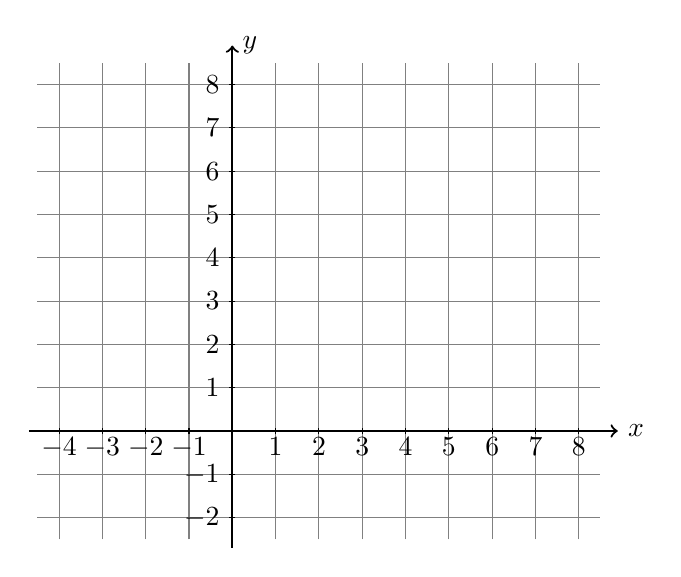
\begin{tikzpicture}[scale=0.55]

\draw [thin, color=gray, xstep=1.0cm, ystep=1.0cm] (-4.5,-2.5) grid (8.5,8.5);

\foreach \x in {-4,-3,-2,-1,1,2,3,4,5,6,7,8}
\draw[shift={(\x,0)}, color=black] (0pt,-2pt) -- (0pt,2pt) node[below] {$\x$};

\foreach \y in {-2,-1,1,2,3,4,5,6,7,8}
\draw[shift={(0,\y)}, color=black] (2pt,0pt) -- (-2pt,0pt) node[left] {$\y$};

\draw [thick, ->] (-4.7,0) -- (8.9,0) node [right] {$x$};
\draw [thick, ->] (0,-2.7) -- (0,8.9) node [right] {$y$};

\end{tikzpicture}
\end{center}
\end{figure}

\newpage

%--- Problem 2: reflections and stretches ---
%--- Source: informed by AA SL 2.11 stretch/reflection items ---
\item[2.] \textbf{Reflections and stretches.} Again start from $f(x)=\dfrac{1}{x}$.

\begin{enumerate}[label=(\alph*), itemsep=0.3cm]
  \item Write down the equation of the image of $f$ after a \emph{reflection in the
  $x$-axis}.

  \vspace{0.8cm}

  \item Write down the equation of the image of $f$ after a \emph{vertical stretch
  with scale factor $2$}.

  \vspace{0.8cm}

  \item Consider $\displaystyle g(x)=\dfrac{-2}{x-1}$.

  \begin{enumerate}[label=(\roman*), itemsep=0.2cm]
    \item Describe a sequence of transformations that maps $f$ onto $g$.

    \vspace{1.4cm}

    \item State the equations of the two asymptotes of $g$.

    \vspace{0.9cm}

    \item Find the coordinates of any axis intercepts of $g$.

    \vspace{1.3cm}

    \item Sketch $g$ on the axes below (dashed asymptotes); check with your GDC.
  \end{enumerate}
\end{enumerate}

\begin{figure}[H]
\begin{center}
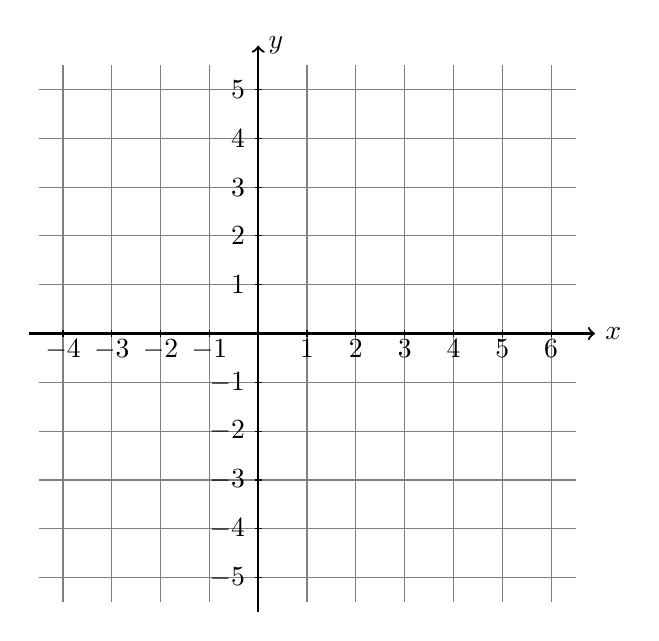
\begin{tikzpicture}[scale=0.62]

\draw [thin, color=gray, xstep=1.0cm, ystep=1.0cm] (-4.5,-5.5) grid (6.5,5.5);

\foreach \x in {-4,-3,-2,-1,1,2,3,4,5,6}
\draw[shift={(\x,0)}, color=black] (0pt,-2pt) -- (0pt,2pt) node[below] {$\x$};

\foreach \y in {-5,-4,-3,-2,-1,1,2,3,4,5}
\draw[shift={(0,\y)}, color=black] (2pt,0pt) -- (-2pt,0pt) node[left] {$\y$};

\draw [thick, ->] (-4.7,0) -- (6.9,0) node [right] {$x$};
\draw [thick, ->] (0,-5.7) -- (0,5.9) node [right] {$y$};

\end{tikzpicture}
\end{center}
\end{figure}

\newpage

%--- Problem 3: (ax+b)/(cx+d) rewritten as a transformation of 1/x ---
%--- Source: informed by 25M.1.SL.TZ2.3 f(x)=(3x-2)/(2x+1) and 8-2CW Problem 1 ---
\item[3.] \textbf{From $\dfrac{ax+b}{cx+d}$ to a transformation.} Consider
$\displaystyle f(x)=\dfrac{2x+7}{x+3}$, \ $x\ne -3$.

\begin{enumerate}[label=(\alph*), itemsep=0.3cm]
  \item Use division (or otherwise) to show that
  $\displaystyle f(x)=2+\dfrac{1}{x+3}$.

  \vspace{1.7cm}

  \item Hence describe $f$ as a sequence of transformations of the parent
  function $y=\dfrac{1}{x}$.

  \vspace{1.1cm}

  \item Write down the equations of the asymptotes, and find the $x$- and
  $y$-intercepts of $f$.

  \vspace{1.8cm}

  \item Sketch $f$ on the axes below. Label the asymptotes (dashed) and the
  intercepts.
\end{enumerate}

\begin{figure}[H]
\begin{center}
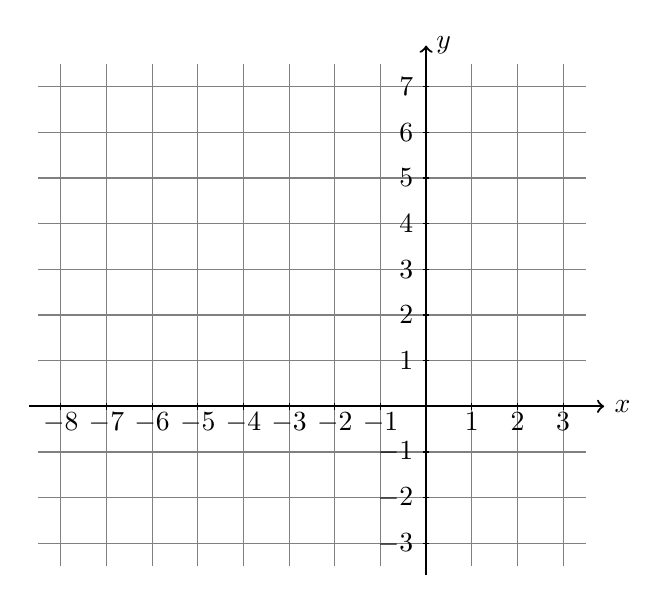
\begin{tikzpicture}[scale=0.58]

\draw [thin, color=gray, xstep=1.0cm, ystep=1.0cm] (-8.5,-3.5) grid (3.5,7.5);

\foreach \x in {-8,-7,-6,-5,-4,-3,-2,-1,1,2,3}
\draw[shift={(\x,0)}, color=black] (0pt,-2pt) -- (0pt,2pt) node[below] {$\x$};

\foreach \y in {-3,-2,-1,1,2,3,4,5,6,7}
\draw[shift={(0,\y)}, color=black] (2pt,0pt) -- (-2pt,0pt) node[left] {$\y$};

\draw [thick, ->] (-8.7,0) -- (3.9,0) node [right] {$x$};
\draw [thick, ->] (0,-3.7) -- (0,7.9) node [right] {$y$};

\end{tikzpicture}
\end{center}
\end{figure}

\newpage

%--- Problem 4: reverse direction — build the function from a description ---
\item[4.] \textbf{Building a function from transformations.} The graph of a
function $g$ is obtained from the parent function $y=\dfrac{1}{x}$ by the following
sequence:

\begin{center}
a vertical stretch with scale factor $3$, \ then a translation $2$ units right and
$1$ unit down.
\end{center}

\begin{enumerate}[label=(\alph*), itemsep=0.3cm]
  \item Write down an expression for $g(x)$.

  \vspace{2.0cm}

  \item State the equations of the two asymptotes of $g$.

  \vspace{1.4cm}

  \item Find the coordinates of the $x$-intercept and the $y$-intercept of $g$.

  \vspace{3.0cm}

  \item Use your GDC to verify your graph, and write down the value of $g(8)$.

  \vspace{2.0cm}
\end{enumerate}

\newpage

%--- Problem 5: rapid identification drill ---
\item[5.] \textbf{Quick identification.} For each function, describe fully the
transformation(s) of the parent function $y=\dfrac{1}{x}$ that produce it, and
state the equations of its two asymptotes.

\begin{enumerate}[label=(\alph*), itemsep=0.7cm]
  \item $\displaystyle y=\dfrac{1}{x-5}$
  \vspace{1.4cm}

  \item $\displaystyle y=\dfrac{1}{x}-4$
  \vspace{1.4cm}

  \item $\displaystyle y=\dfrac{4}{x}$
  \vspace{1.4cm}

  \item $\displaystyle y=-\dfrac{1}{x}$
  \vspace{1.4cm}

  \item $\displaystyle y=\dfrac{1}{x+2}+1$
\end{enumerate}

\newpage

%--- Problem 6: transformations of a general given graph ---
%--- Source: informed by 24M.1.SL.TZ2.1 / 21M.1.SL.TZ1.1 (graph-of-f transformation type) ---
\item[6.] \textbf{Transforming a given graph.} Transformations work on
\emph{any} function, not only the reciprocal. The diagram shows the graph of a
function $y=f(x)$, made of three straight segments through the marked points.

\begin{figure}[H]
\begin{center}
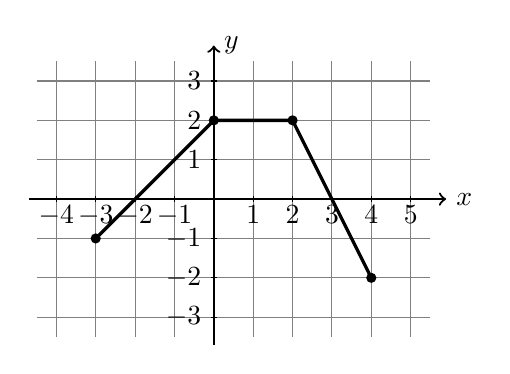
\begin{tikzpicture}[scale=0.5]

\draw [thin, color=gray, xstep=1.0cm, ystep=1.0cm] (-4.5,-3.5) grid (5.5,3.5);

\foreach \x in {-4,-3,-2,-1,1,2,3,4,5}
\draw[shift={(\x,0)}, color=black] (0pt,-2pt) -- (0pt,2pt) node[below] {$\x$};

\foreach \y in {-3,-2,-1,1,2,3}
\draw[shift={(0,\y)}, color=black] (2pt,0pt) -- (-2pt,0pt) node[left] {$\y$};

\draw [thick, ->] (-4.7,0) -- (5.9,0) node [right] {$x$};
\draw [thick, ->] (0,-3.7) -- (0,3.9) node [right] {$y$};

% graph of f: segments through (-3,-1), (0,2), (2,2), (4,-2)
\draw [very thick] (-3,-1) -- (0,2) -- (2,2) -- (4,-2);
\foreach \pt in {(-3,-1),(0,2),(2,2),(4,-2)}
  \node[circle, fill, inner sep=1.3pt] at \pt {};

\end{tikzpicture}
\end{center}
\end{figure}

\begin{enumerate}[label=(\alph*), itemsep=0.3cm]
  \item Write down the values of $f(0)$ and $f(2)$.

  \vspace{1.0cm}

  \item The graph of $g$ is obtained from $f$ by the transformation
  $g(x)=f(x)-3$. Describe this transformation in words, and write down the
  coordinates of the image of the point $(0,2)$.

  \vspace{1.5cm}

  \item On the axes below, sketch the graph of $y=f(x-1)$ (a translation of $f$).
  Mark the images of the four labelled points.
\end{enumerate}

\begin{figure}[H]
\begin{center}
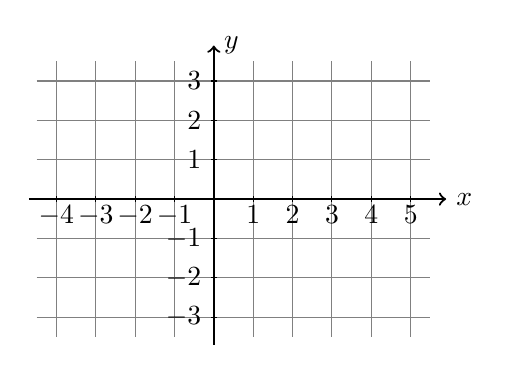
\begin{tikzpicture}[scale=0.5]

\draw [thin, color=gray, xstep=1.0cm, ystep=1.0cm] (-4.5,-3.5) grid (5.5,3.5);

\foreach \x in {-4,-3,-2,-1,1,2,3,4,5}
\draw[shift={(\x,0)}, color=black] (0pt,-2pt) -- (0pt,2pt) node[below] {$\x$};

\foreach \y in {-3,-2,-1,1,2,3}
\draw[shift={(0,\y)}, color=black] (2pt,0pt) -- (-2pt,0pt) node[left] {$\y$};

\draw [thick, ->] (-4.7,0) -- (5.9,0) node [right] {$x$};
\draw [thick, ->] (0,-3.7) -- (0,3.9) node [right] {$y$};

\end{tikzpicture}
\end{center}
\end{figure}

\end{enumerate}
\end{document}
